The next LHC run for taking data (Run 3) will require more resources than the
Worldwide LHC Computing Grid (WLCG) can possibly provide. Currently, PanDA WMS
uses more than 100,000 cores at over 100 Grid sites, with a peak performance of
0.3 petaFLOPS. This capacity will be sufficient for the planned analysis and
data processing, but it will be insufficient for the Monte Carlo production
workflow and any extra activity. To alleviate these challenges, ATLAS is engaged
in a program to expand the current computing model to include additional
resources such as the opportunistic use of supercomputers as well as commercial
and academic clouds.


% -----------------------------------------------------------------------------
\subsection{Use of Supercomputers with PanDA}
\label{ssec:panda-supercomputers}

Modern supercomputers have been designed mainly to support parallel computation
that requires runtime communication. Job execution is parallelized across
multiple cores, each core calculating a small part of the problem and
communicating with other cores via a message passing interface (MPI).
Accordingly, supercomputers have large number of worker nodes, connected through
a high-speed, low-latency dedicated network. Each worker node has multicore
CPUs, usually augmented with massively parallel Graphics Processing Units (GPUs)
or other types of specialized coprocessors.

PanDA WMS has been designed to support distributed Grid
computing\sergeynote{specifically "distributed Grid computing"}\mtnote{done.}.
Executing ATLAS workloads or workflows involves concurrent and/or sequential
runs of possibly large amount of jobs, each requiring no or minimal
parallelization and no runtime communication. Thus, computing infrastructure
like WLCG have been designed to aggregate large amount of computing resources
across multiple sites.
%, often geographically dislocated.
\sergeynote{geographically distributed?}\mtnote{Better?} While each site may
deploy runtime message-passing capabilities, usually these are not used to
perform distributed computations.

There are at least two approaches to enable PanDA WMS to execute ATLAS workloads
or workflows on supercomputers: (i) using the subset of resources and
capabilities shared by both supercomputers and WLCG; (ii) reconciling the
parallel and distributed computing paradigms by means of dedicated abstractions.
The former is a pragmatic approach that enables the execution of specific
workloads by prototyping single-point solutions. The latter is a principled
approach, better suited for a production-grade solution, capable of supporting
general-purpose workloads and workflows on both supercomputers and Grid
infrastructures. These two approaches are not mutually exclusive: developing a
single-point solution gives the opportunity to better understand the problem
space, supporting the creation of abstractions for the integration of computing
paradigms.

This section illustrates the design and architecture of a job broker prototyped
by the PanDA team. This broker supports execution of part of the ATLAS
production Monte Carlo workflow on Titan, a leadership-class supercomputer
managed by the Oak Ridge Leadership Computing Facility (OLCF) at the Oak Ridge
National Laboratory (ORNL). After an analysis of the results obtained and the
lessons learned, the following section introduces the design and first
experimental characterization of a next generation executor (NGE). NGE is
designed to abstract resources and capabilities, enabling the concurrent
execution of both parallel and distributed computing on generic high performance
computing (HPC) machines.


% -----------------------------------------------------------------------------
\subsection{Interfacing PanDA with Titan}
\label{ssec:panda-titan}

The Titan supercomputer, current number three
% (number one from November 2012 until June 2013)
on the Top 500 list~\cite{top500}, is a Cray XK7 system with 18,688 work nodes
and a total of 299,008 CPU cores. Each work node has an AMD Opteron CPU, a
Nvidia Tesla GPU, 32 GB of RAM and no local storage, though a 16 GB RAM disk can
be set up. Work nodes use Cray’s Gemini interconnect for inter-node MPI
messaging. Titan is served by the Spider II~\cite{spider2}, a Lustre filesystem
with 32 PB of disk storage, and by a 29 PB HPSS tape storage system. Titan’s
work nodes run Compute Node Linux, a run time environment based on SUSE Linux
Enterprise Server.

% Titan, was the first large-scale system to use a hybrid architecture that
% utilizes worker nodes with both AMD 16-core Opteron 6274 CPUs and NVIDIA Tesla
% K20 GPU accelerators.
% This hybrid design provides improved energy efficiency, as well as an order of
% magnitude in computational capacity over its predecessor.

Titan offers to its users login nodes and data transfer nodes (DTNs). Users have
to log into one of these nodes via ssh to submit jobs to Titan's PBS scheduler.
Titan's authentication and authorization model is based on two-factor
authentication with a RSA SecurID key, generated every 30 seconds. Login nodes
and DTNs are the only nodes with out/inbound wide area network connectivity.
Work nodes have only local network access. Data staging is supported via the
DTNs, from the wide area network and the OLCF high performance storage system
(HPSS). DTNs are shared across all Titan's users that can schedule jobs to a
dedicates batch system to automate data staging. Fair-share policies are in
place both for the batch system and for the use of DTN resources.

Titan's architecture, configuration and policies poses several challenges to the
integration with PanDA. PanDA Pilot requires to contact the Job Dispatcher
module of the PanDA Server to pull jobs to execute. Titan's work nodes do not
offer outbound network connectivity, making the current deployment model of
PanDA pilots unfeasible. Titan does not support PanDA's security model based on
certificates and virtual organizations, making the PanDA's approach to identity
management also unfeasible. While DTNs offer wide area network data transfer, an
integration with ATLAS DDM is beyond the functional and administrative scope of
the current prototyping phase. Finally, the specific characteristics of the
execution environment, especially the absence of local storage on the work nodes
and modules tailored to Compute Node Linux, require reengineering of ATLAS
application frameworks.

Currently, no HEP application can benefit from Titan's GPUs but some
computationally-intensive and non memory-intensive tasks can be offloaded from
the Grid to Titan's large amount of cores. Further, when HEP tasks can be
partitioned to independent jobs, Titan work nodes can be used to execute up to
16 concurrent jobs' payload, one for each available core. Given these
constraints and challenges, the type of task most suitable for execution at the moment on Titan is Monte Carlo
% event generation and
detector simulation.
% Both types of task are
This type of task is mostly computational-intensive, requiring less than 2GB of
RAM at runtime and with small input data requirements. Detector simulation tasks
in ATLAS account for XX--XX\% of all jobs on WLCG, corresponding to X/X of the
current Grid capacity.\mtnote{Please provide numbers to replace `XX' and,
possibly, a diagram illustrating detector simulation stats compared to the whole
ATLAS computation activity.}

% The event generation in ATLAS accounts for 10--15\% of all jobs on WLCG,
% corresponding to 2/3 of the current Grid capacity.


% Event generation and
Detector simulation is part of the ATLAS production Monte Carlo (MC) workflow
(also known as MC production
chain)~\cite{rimoldi2006atlas,de2013delphes,ritsch2014atlas}. The MC workflow
consists of four main stages: event generation, detector simulation,
digitization, and reconstruction. Even generation creates sets of particle
four-momenta via different generators, e.g., PYTHIA~\cite{sjostrand2006pythia}
and HERWIG~\cite{corcella2001herwig}. The detector simulator is called
Geant4~\cite{agostinelli2003geant4} and simulates the interaction of these
particles with the sensitive material of the ATLAS detector. Each interaction
creates a so-called hit and all hits are collected and passed on for
digitalization where hits are further process to mimic the readout of the
detector. Finally, reconstruction operates local pattern recognition, creating
high-level objects like particles and jets.

% While this is different from the HEP computing paradigm, where jobs are
% independent, it still shares common features such as the use of
% parallelization. It is not a requirement that HPC machines are able to run
% any possible task, nor is it relevant how many kinds of job types that can be
% run. What matters is the total number of cycles that can be offloaded from
% the Grid.

% Standard ATLAS workflow can not be easily ported to supercomputers due to
% several complications such as specialized worker node setups, no outbound
% network connections, limited memory per node, custom operating systems, etc. A
% reorganization of the standard workflow is therefore needed.

% -----------------------------------------------------------------------------
\subsection{PanDA Broker on Titan}
\label{ssec:panda_titan}

The lack of wide area network connectivity on Titan's work nodes is the most
relevant challenge for integrating PanDA WMS and Titan. Without connectivity,
Panda Pilots cannot be scheduled on work nodes because they would not be able to
communicate with PanDA Server and therefore pull and execute jobs. This makes
impossible to port PanDA Pilot to Titan while maintaining the defining feature
of the pilot abstraction: decoupling resource acquisition from workload
execution via multi-stage scheduling.

The unavailability of pilots is a potential drawback when executing distributed
workloads like MC
% event generation and
detector simulation. Pilots are used to increase the throughput of distributed
workloads: while pilots have to wait in the supercomputer's queue, once
scheduled, they can pull and execute jobs independently from the system's queue.
Jobs can be concurrently on every core available to the pilot and multiple
generations of concurrent executions can be performed until the pilot's walltime
is exhausted. This is particularly relevant for machines like Titan where queue
policies privilege parallel jobs on the base of the number of work nodes they
request: the higher the number of nodes, the shorter the amount of queue time
(modulo fair share policies).

% MC event generation and simulation tasks can be executed without pilots but
% the time spent waiting in the queue would be too large compared to the
% execution time of each task.

Titan’s backfill functionality offers the opportunity to avoid the overhead of
queue wait times without using pilot abstraction. Backfill availability is the
number of work nodes that cannot be used by any of the jobs already queued on
Titan: All queued jobs are either too large or their walltime is too long. At
any point in time, Titan’s Moab scheduler can be queried for backfill
availability. Based upon the result of this query, a job can be shaped to
request no more than the backfill availability, and when submitted as such is
usually scheduled immediately spending almost no time in the queue.

Compared to pilots, backfill has the disadvantage of limiting the amount of work
nodes that can be requested. Pilots are normal jobs: they can request as many
work nodes for as much time as a queue can offer. On the contrary, jobs sized on
the basis of backfill information availability \jhanote{should be resource
availability or backfill queue information?}\mtnote{AFAIH, there is no dedicated
queue to backfill} depend on the number % amount
of work nodes that cannot be given to any other job. any other job in the
Titan's queue\sergeynote{any other job currently in the Titan's
queue?}\mtnote{Better?}. Usually, backfill availability is a fraction of the
total capacity of the queue but the size of Titan mitigates this limitation.
Every year, about 10\% of Titan's capacity remains
unused~\cite{titan_utilization}, corresponding to an average of 30,000 unused
cores. This equals approximately 270M core hours per year, roughly 30\% of the
overall capacity of WLCG.

% A system that can use those temporarily free work nodes with smaller
% scale tasks would be very valuable. For this reason, Titan offers backfill
% functionalities: users can interrogate Titan's Moab scheduler about how many
% free nodes are currently available and for how long. If a user submit a
% requestvfor that number of nodes and walltime, queue time will be minimal.

\mtnote{Please feel free to add details about backfill as needed.}
\mtnote{Please note: I know the following departs for the current name given to
the PanDA subsystem installed on Titan. I think there is a good reason to call
it a broker instead of a pilot, and I think I explained it in the previous
paragraphs. Please  take this just as a suggestion, something I would like to
discuss in our meeting.} \sergeynote{It's not a pilot in conventional sense. I
call it an agent. It just happened that we were able to use full PanDA pilot's
code base to serve our purposes on Titan. that's why, by inertia, we still call
it a pilot.}\mtnote{Thank you. We would have a problem calling it `agent' as we
use that term to name the pilot of NGE. Would PanDA Broker work?}\mtnote{Sergey
agreed that we should not use `pilot'. He is quite convinced by `broker' but we
are both open to better suggestions.}

Given the communication requirements of PanDA Pilots and the unused capacity of
Titan, PanDA pilot was redesigned to serve as a job broker on Titan. Architected
as a stand-alone service to be executed on a DTN, this prototype called `PanDA
Broker' implements functionalities to: (i) interrogate Titan about backfill
availability; (ii) pull MC jobs and events; (iii) wrap jobs' payload into PBS
MPI jobs; (iv) submitting MPI PBS jobs to Titan's PBS batch system and monitor
their execution;\sergeynote{Monitor job state and state transitions using
SAGA}\mtnote{Better?} and (v) staging input/output files. Backfill querying,
payload wrapping, and job submission required a new implementation while job and
events pulling, and file staging were mostly inherited from PanDA Pilot.

\begin{figure}
  \begin{center}
    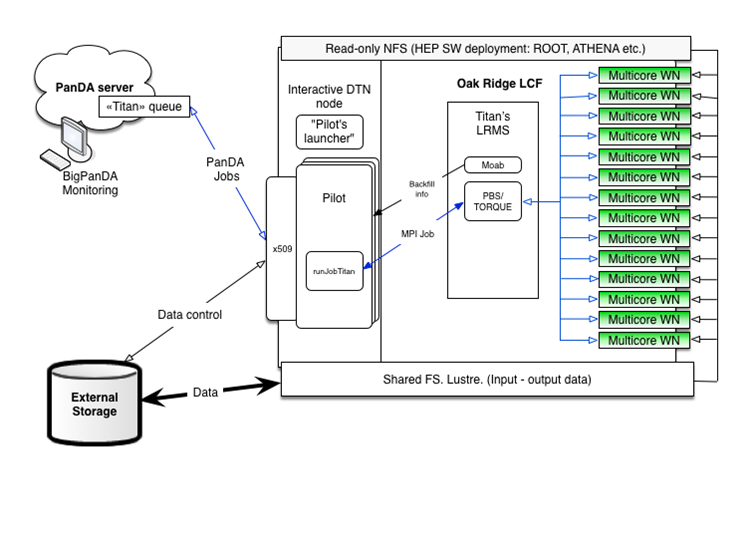
\includegraphics[width=\columnwidth]{figures/PanDA_setup_at_OLCF.png}
    \caption{Schematic view of the PanDA Broker.}
  \end{center}
\label{fig:panda_broker}
\end{figure}

Backfill querying is performed via a dedicated Moab command while a tailored
Python MPI script is used to wrap job's payload. This MPI wrapper serves as a
``container'' for non-MPI jobs, enabling execution of unmodified Grid-centric
jobs on Titan. Typically, a MPI wrapper is workload-specific as it sets up the
execution environment for a specific payload. This involves organization of
worker directories, data management, optional input parameters modification, and
cleanup on exit. Upon submission, a copy of the MPI wrapper runs on every
available work node. Each script knows its MPI rank (an index that runs from
zero to a maximum number of nodes or script copies) as well as the total number
of ranks in the current submission. When activated on worker nodes, each copy of
the wrapper script starts the execution of the payload in a subprocess and waits
until its completion.

MPI wrappers are submitted to Titan's PBS batch system via
RADICAL-SAGA~\cite{radical-saga}, a Python module, compliant with the OGF GFD.90
SAGA specification~\cite{saga-spec}. The Simple API for Grid Applications (SAGA)
offers a unified interface to diverse job schedulers and file transferring
services. In this way, SAGA provides an interoperability layer that lowers the
complexity of using distributed infrastructures. Behind the API façade,
RADICAL-SAGA implements a adaptor architecture: each adaptor interface the SAGA
API with different middleware systems and services, including the batch
scheduler of Titan.

The data staging capabilities of the PanDA Broker are implemented via a file
system that is shared among DTNs and work nodes. The input files required by the
payload are downloaded via the ATLAS DDM service and then stored in a directory
on the shared filesystem. The MPI wrapper setup process includes making the
location of these files available to the payload. The PanDA Broker can locate
the Payloads' output files on the shared filesystem and transfer them from Titan
to the ATLAS Tier 1 computing center at Brookhaven National Lab (BNL) or any
other Grid site.

Once deployed, every PanDA Broker supports the execution of MC detector
simulation on Titan in 8 steps: (i) PanDA Broker queries Titan's Moab scheduler
about current backfill availability; (ii) the PanDA Broker queries the Job
Dispatcher module of the PanDA server for jobs that have been bound to Titan by
JEDI; (iii)  the PanDA Broker requests to the Data Service module of the PanDA
Server what input data these jobs require and transfer the files to the DTN via
the ATLAS DDM service; (iv) the PanDA Broker creates a PBS MPI script, wrapping
enough jobs' payload to fit backfill availability; (v) the PanDA Broker submits
the PBS MPI script to the Titan's PBS batch system via RADICAL-SAGA; (vi) upon
execution on the worker node(s), the MPI script creates a ramdisk and configure
AthenaMP to execute the wrapped payload; (vii) the payload is executed into
dedicated processes, 16 for each work node, 1 for each available core; (viii)
upon completion of the MPI script, the PanDA Broker locates the output on the
shared NFS filesystem and transfer it to BNL ATLAS Tier 1 computing centre.

% from the Job Dispatcher module of PanDA Server (as done by a PanDA Pilot);
% (iii) downloading events via PanDA Server's Data Service from ATLAS DDM to
% Titan's DTN; (iv) wrap the Geant4 payload into a PBS job; (v) submit jobs to
% Titan's PBS batch scheduler;

% Integration with Titan is the current focus for PanDA developers.

% The project aims to integrate Titan with the PanDA system using an updated
% PanDA Pilot that runs on the front-end node and submits ATLAS payloads to the
% worker nodes using the local batch system (PBS) via the SAGA (Simple API for
% Grid Applications) interface~\cite{SAGA}. This solves several complications
% of running on HPC worker nodes, including the lack of connectivity to outside
% world. The pilot can communicate with the PanDA server from the front-end
% machine.

% \paragraph*{HPC Backfill} HPC facilities are geared towards large scale jobs
% by design. Time allocation on an HPC is competitive and large projects are
% often preferred. About 10\% of capacity on a typical HPC machine is unused
% due to mismatches between job sizes and available resources. The worker nodes
% sit idle because there are not enough of them or they do not have enough time
% to handle a large scale computing job. On a machine of the scale of Titan,
% these 10\% correspond to estimated 300M core hours per year. A system that
% can occupy those temporarily free nodes with smaller scale tasks would be
% very valuable.

% This offers a great possibility for PanDA to harvest the opportunistic
% resources on Titan and use a similar mechanism on other HPCs. Functionality
% has been added to the PanDA Pilot to collect information about available
% unused worker nodes on Titan in real time.

% First test of the system were quite successful and show great promise in
% increasing the resource utilization on Titan.
